%%
%% Template chap1.tex
%%

\chapter{Evaluation of Social Recommendation Systems}

In this chapter we first discuss our Facebook Link Recommendation
(LinkR) application and then proceed to discuss how it can be
evaluated using general principles of evaluation used in the
machine learning and information retrieval fields.

\section{Facebook}

Facebook is a social networking service that is currently the largest
in the world. As of July 2011 it had more that 750 million active
users. Users in Facebook create a profile and establish ``friend''
connections between users to establish their social network. Each user
has a ``Wall'' where they and their friends can make posts to.  These
posts can be links, photos, status updates, etc.  Items that have been
posted by a user can be ``liked'', shared, or commented upon by other
users.  An example of a link post on a Wall that had been liked
by others was provided previously in Figure~\ref{fig:ex_link}.

%\begin{figure}[h]
%\centering
%\subfigure{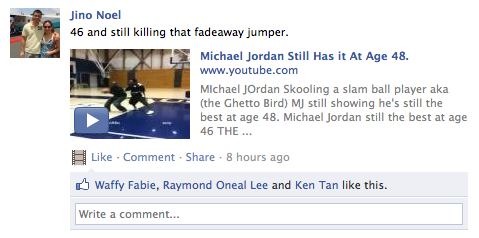
\includegraphics[scale=0.50]{img/posted-link.png}}
%\subfigure{
\includegraphics[scale=0.50]{img/posted-link.eps}}
%\caption{A link posted by the author that has been liked by three other users.}
%\end{figure}

This thesis seeks to find out how best to recommend links to
individual users such that there is a high likelihood that they will
``like'' their recommended links.  We do this by creating a
Facebook application (i.e., `Facebook ``App'') that recommends links
to users everyday, where the users may give their feedback on the
links indicating whether they \emph{liked} it or \emph{disliked} it.
We discuss this application in detail next.

\subsection{LinkR}

Facebook allows applications to be developed that can be installed by
their users.  As part of this thesis project, the LinkR Facebook
application was developed.\footnote{The main developer of the LinkR
Facebook App is Khoi-Nguyen Tran, a PhD student at the Australian
National University.  Khoi-Nguyen wrote the user interface and database
crawling code for LinkR.  All of the learning and recommendation
algorithms used by LinkR were written solely by the author for the
purpose of this thesis.}  The functionalities of the LinkR application
are as follows:
\begin{enumerate}
\item{Collect data that have been shared by users and their friends on Facebook.}
\item{Recommend (three) links to the users daily.}
\item{Collect feedback from the users on whether they liked or disliked the recommendations.}
\end{enumerate}

Figure~\ref{fig:linkr_app} shows the Facebook LinkR App as it appears
to users.
\begin{figure}[t!]
\centering
%\subfigure{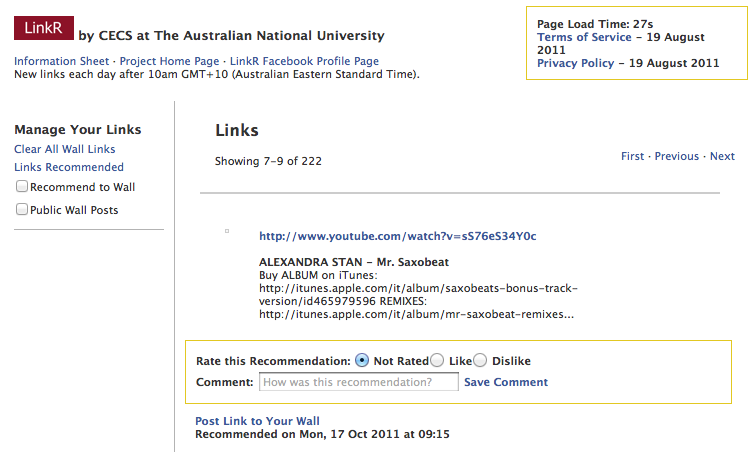
\includegraphics[scale=0.30]{img/linkr.png}}
\subfigure{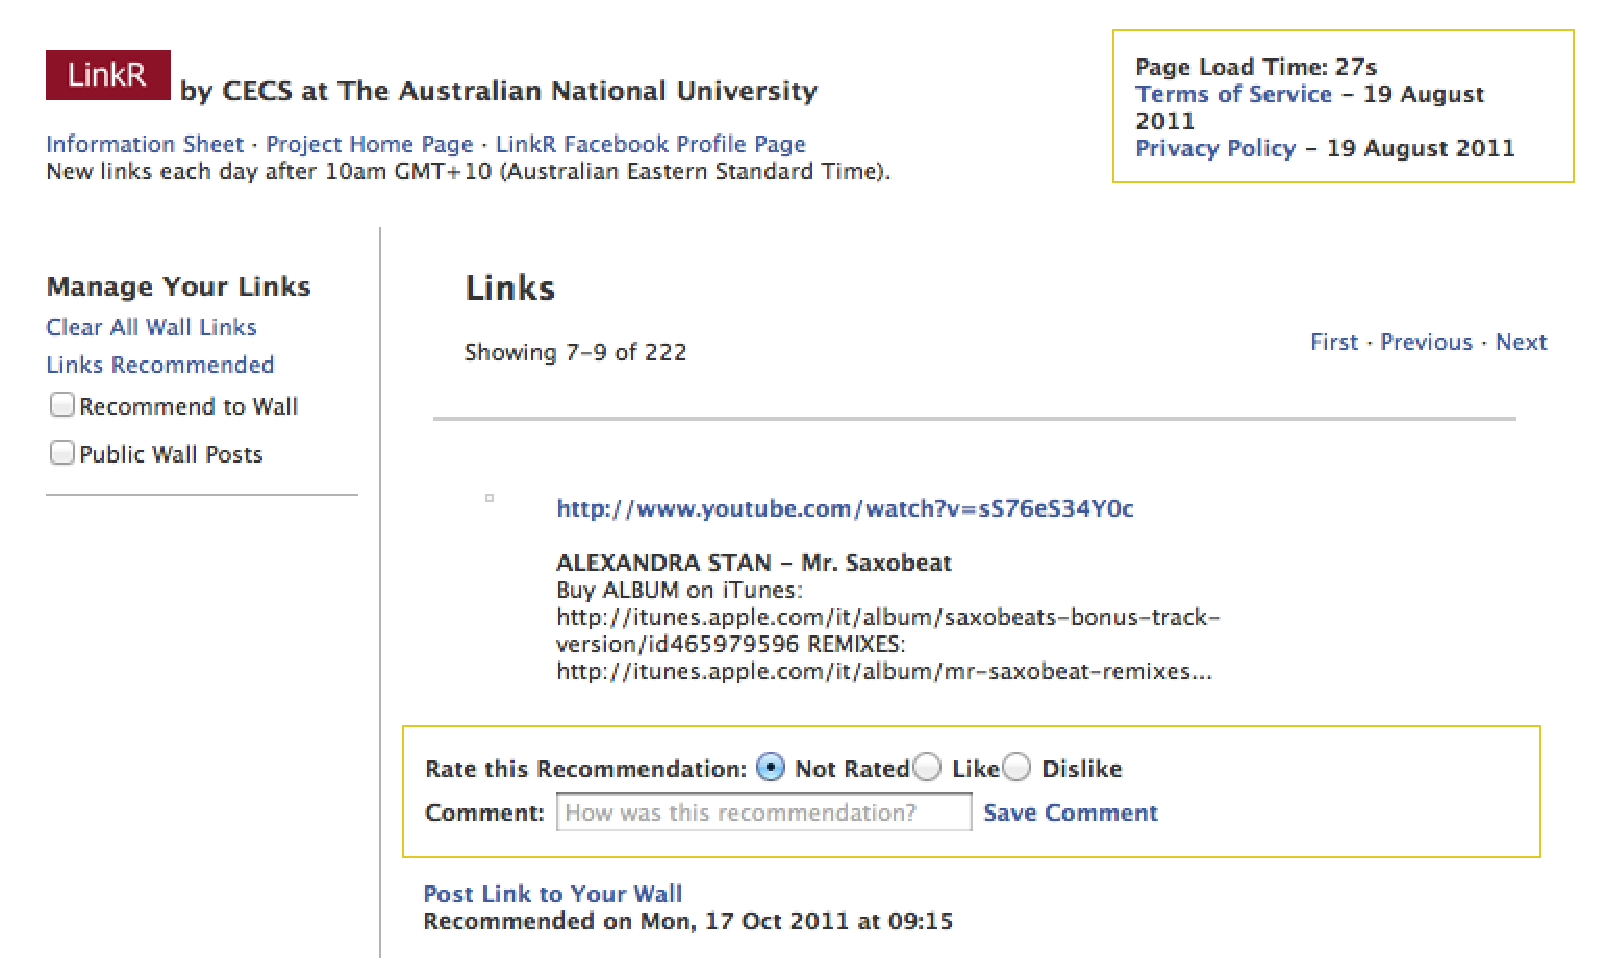
\includegraphics[scale=0.55]{img/linkr.eps}}
\caption{The Facebook LinkR App showing one of the recommendations
as it appears to users of the system.  Users have the option of liking
or disliking a recommendation as well as providing explicit feedback
commentary.}
\label{fig:linkr_app}
\end{figure}

\section{Dataset}

\label{sec:dataset}

Using the LinkR Facebook App developed for this project, we were able
to gather data on 34,245 users and 407,887 links.\footnote{As of
October 18, 2011, 12:15am.}

\subsection{User Data}

Date that are collected and used for the user features are as follows:
\begin{itemize}
\item {Gender:} male or female
\item {Birthday:} year
\item {$\mathit{location}_\mathit{id}$:} an integer ID corresponding
to the user's specific present location (city and country)
\item {$\mathit{hometown}_\mathit{id}$:} an integer ID corresponding
to the user's specific home town (city and country)
\item {$F_{\x,\z} \in \{ 0, 1\}$:} indicator of whether 
users $\x$ and $\z$ are friends.
% Joseph: be specific here...
\item {$\mathit{Int}_{\x,\z} \in \mathbb{N}$:} interactions on
Facebook between users $\x$ and $\z$.
\end{itemize}

\subsection{Link Data}

Data that are used for the link features are:
\begin{itemize}
\item{$\mathit{id}$ of the user who posted the link.}
\item{$\mathit{id}$ of the user on whose wall the link was posted.}
\item{Text description of the link from the user who posted it.}
\item{Text link summary from the metatags on the target link webpage.}
\item{Number of times the link has been liked.}
\item{Number of times the link has been shared.}
\item{Number of comments posted on the link}.
\item {$F'_{\x,\y} \in \{0, 1\}$:} indicator of whether user $\x$ has liked item $\y$.
\end{itemize}
Additionally, links that have been recommended by the LinkR
application have the following extra features:
\begin{itemize}
\item{$\mathit{id}$'s of users who have clicked on the link url.}
\item{Optional ``Like'' or ``Dislike'' rating of the LinkR user on the link.}
\end{itemize}

\subsection{Implicit Dislikes}

Outside of the ``Dislike'' ratings that we are able to get from the
LinkR data, there is no other functionality within Facebook itself
that allows users to explicitly define which link they do not
like. Therefore, we need some way to infer disliked links during
training. During training we consider links that were posted by the
user's friends and which they have not likes as an evidence that they
dislike a link. This is a major assumption since users may have simply
not seen the link, yet they may have actually liked it \emph{if} they
had seen it.  Nevertheless, we find both in our offline and online
evaluations that this assumption allows us to augment our training
data in practice and does help performance despite these caveats.

\section{Evaluation Metrics}
\label{sec:map}

\begin{comment}
This paper uses a lot of different evaluation metric to compare the various algorithms discussed. For the collaboration recommendation algorithms which were run the MovieLens dataset, they were solving a regression problem so we used the Root Mean Squared Error (RMSE) metric which was also used to for the Netflix Prize competition.

\[
RMSE = \sqrt{ \frac{\sum_{i=1}^N{ (r_i - p_i)}^2 }{N}}
\]

where {\bf r} are the true rating values for N movies and {\bf p} are the ratings predicted by the recommendation algorithms.

For the social recommendation algorithms, they are trying to solve a classification problem, so instead of RMSE we use various metrics such as accuracy, precision, recall, f1, and a variant of the Mean Average Precision.  Accuracy is a measure of how accurate the algorithm was in classifying all the items.

\[
Accuracy =  \frac{TP + TN}{TP + TN + FP + FN}
\]
\end{comment}

We define \emph{true positives} (TP) to be the count of relevant items
that were returned by the algorithm, \emph{false positives} (FP) to be the
count of non-relevant items that were returned by the algorithm, \emph{true
negatives} (TN) to be the count of non-relevant items that weren't
returned by the algorithm, and \emph{false negatives} (FN) to be the
non-relevant items that were returned by the algorithm.

\emph{Precision} is a measure of what fraction of items returned by
the algorithm were actually relevant.

\[
Precision = \frac {TP} {TP + FP}
\]

\begin{comment}
Recall is the measure of what fraction of all relevant items items were actually returned by the algorithm.

\[
Recall = \frac {TP} {TP + FN}
\]

The F1 score is another measure of an algorithms accuracy, and is calculated as a weighted average between precision and recall.

\[
F1 = 2 \times \frac{precision \times recall}{precision + recall}
\]
\end{comment}

For some problems, results are returned as a ranked list. The position
of an item in the list must also be evaluated, not just whether the
item is in the returned list or not. A metric that does this is
\emph{average precision} (AP), which computes the precision at every
position in a ranked sequence of documents. $k$ is the rank in a
sequence of retrieved documents, $n$ is the number of retrieved
documents, and $P(k)$ is the precision at cut-off $k$ in the
list. $rel(k)$ is an indicator function equalling 1 if the item at
position $k$ is a relevant document, and 0 otherwise. The average
precision is then calculated as follows:

\[
AveP = \frac{\sum_{k=1}^n(P(k) \times rel(k))}{\text{number of relevant problems}}
\]

The main metric we use in this paper is the \emph{mean average
precision} (MAP). Since we make a recommendation for each user, these
recommendations can be viewed as a separate problem per user, and
evaluate the AP for each one. Getting the mean of APs across all users
gives us an effective ranking metric for the entire recommendation system:

\[
MAP = \frac{\sum_{u=1}^U AveP(u)}{\text{number of users}}
\]

\section{Training and Testing Issues}

\subsection{Training Data}

Because of the sheer size of the Facebook data, it was impractical to
run training and recommendations over the entire dataset. To keep the
runtime of our experiments within reason, we used only the most recent
four weeks of data for training the recommenders. This also helps
alleviate some temporal aspects of the user's changing preferences,
i.e., what the user liked last year may not be the same as what he or
she likes this year. We also distinguish between the three types of
link like/dislike data we can get from the dataset:

\begin{itemize}
\item {ACTIVE: The explicit "Like" and "Dislike" rating that a LinkR
user gives on links recommended by the LinkR application. In addition
to this, a click by a user on a recommended link also counts as a like
by that user on that particular link.  This data is only available for
LinkR users as it is specific to the LinkR App.}
\item {PASSIVE: The list of likes by users on links in the Facebook data and the inferred dislikes detailed above.  This data can be collected from all users (App users and non-App users).}
\item{UNION: Combination of the ACTIVE and PASSIVE data.}
\end{itemize}

\subsection{Live Online Recommendation Trials}

For the recommendations made to the LinkR application users, we select
only links posted in the most recent two weeks that the user has not
liked. We use only the links from the last two weeks since an informal
user study has indicated a preference for recent links.  Furthermore,
older links have a greater chance of being outdated and are also
likely to represent broken links that are not working anymore. We have
settled on recommending three links per day to the LinkR users and
according to the survey done at the end of the first trial, three
links per day seems to be the generally preferred number of
daily recommendations.

For the live trials, Facebook users who installed the LinkR
application were \emph{randomly assigned one of four algorithms in
each of the two trials}. Users were not informed which algorithm was
assigned to them to remove any bias. We distinguish our recommended
links into two major classes, links that were posted by the LinkR
user's friends and links that were posted by users other than the
LinkR user's friends. The LinkR users were encouraged to rate the
links that were recommended to them, and even provide feedback
comments on the specific links. In turn these ratings became part of
the training data for the recommendation algorithms, and thus were used
to improve the performance of the algorithms over time. Based on the
user feedback, we filtered out non-English links and links without any
descriptions from the recommendations to prevent user annoyance.

At the end of the first trial, we conducted a user survey with the
LinkR users to find out how satisfied they were with the
recommendations they were getting.

\begin{figure}
\centering
%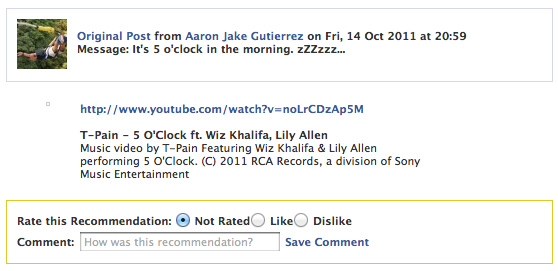
\includegraphics[scale=0.5]{img/linkr_rating.png}
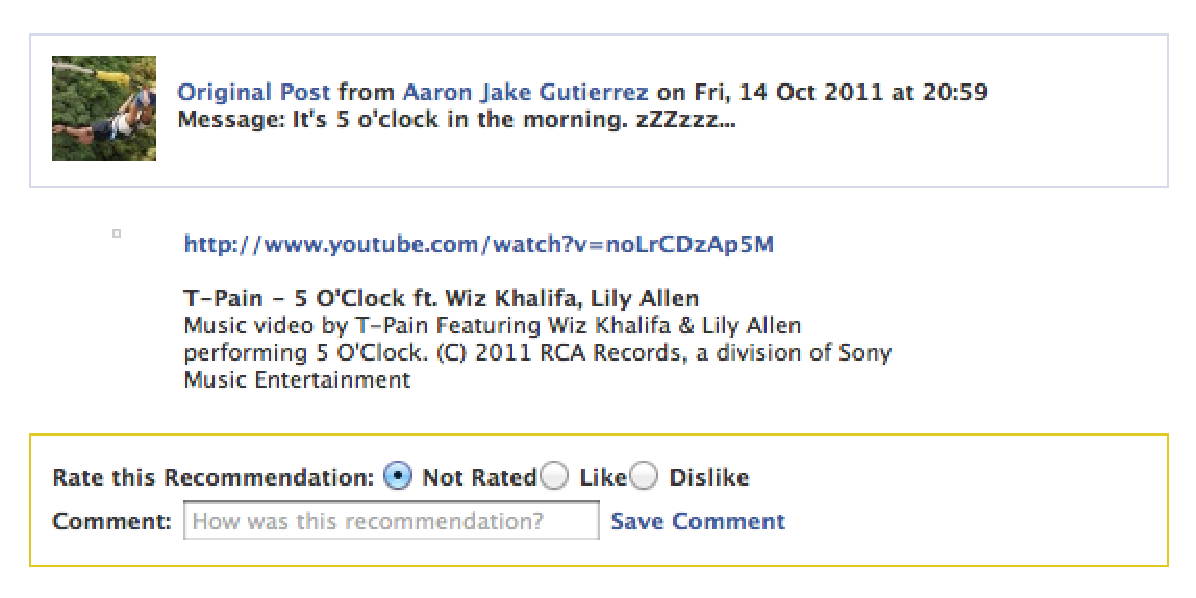
\includegraphics[scale=0.7]{img/linkr_rating.eps}
\caption{Screenshot of a recommendation made by the LinkR application with the rating and feedback options.  In contrast to Figure~\ref{fig:linkr_app}, which showed a recommendation from a non-friend, this example shows a recommendation from a friend, where we are then able to also provide the friend's name and comment text along with the link recommendation.}
 \end{figure}
 
\subsection{Test Data}

Similar to our selection for training data, the test data used for our
passive experiment also uses only the most recent 4 weeks of data. We
distinguish the test data into the following classes:

\begin{itemize}
\item{FB-USER-PASSIVE: The PASSIVE like/dislike data for all Facebook users in the dataset.}
\item{APP-USER-PASSIVE: The PASSIVE like/dislike data for only the LinkR application users.}
\item{APP-USER-ACTIVE-FRIENDS: The ACTIVE like/dislike data for the LinkR users, but only for friend recommended links.}
\item{APP-USER-ACTIVE-NON-FRIENDS: The ACTIVE like/dislike data for the LinkR users, but only for non-friend recommended links.}
\item{APP-USER-ACTIVE-ALL: The entire active like/dislike data for the LinkR users.}
\end{itemize}

During PASSIVE experiments, we simply selected which combination of
training data and testing data to use.  This helped us to determine
which training-test data combination best reflected the results of the
live trials as we discuss in the next chapter.
%Eventually, it was found that using UNION data for training and
%testing on APP-USER-ACTIVE-ALL best reflected the results of the live
%trials.
In cases where training and testing data overlap, i.e., training on
PASSIVE and testing on APP-USER-PASSIVE, we sample a random 20\%
subset of the training data per user for testing. These links are then
removed from the training data to ensure that there are no common
links between the training data and the test data.  When there is no
train/test overlap, i.e., training only on PASSIVE and testing only on
ACTIVE, then we use the full respective datasets for training and
testing.
